%%%%%%%%%%%%%%%%%%%%%%%%%%%%%%%%%%%%%%%%%
% Beamer Presentation
% LaTeX Template
% Version 1.0 (10/11/12)
%
% This template has been downloaded from:
% http://www.LaTeXTemplates.com
%
% License:
% CC BY-NC-SA 3.0 (http://creativecommons.org/licenses/by-nc-sa/3.0/)
%
%%%%%%%%%%%%%%%%%%%%%%%%%%%%%%%%%%%%%%%%%

%----------------------------------------------------------------------------------------
%	PACKAGES AND THEMES
%----------------------------------------------------------------------------------------

\documentclass[UTF8,aspectratio=169,14pt]{ctexbeamer}

\usepackage{hyperref}
\hypersetup{
	colorlinks=true,
	linkcolor=red,
	anchorcolor=blue,
	citecolor=green
}

\mode<presentation> {
	
	% The Beamer class comes with a number of default slide themes
	% which change the colors and layouts of slides. Below this is a list
	% of all the themes, uncomment each in turn to see what they look like.
	
	%\usetheme{default}
	%\usetheme{AnnArbor}
	%\usetheme{Antibes}
	%\usetheme{Bergen}
	%\usetheme{Berkeley}
	%\usetheme{Berlin}
	%\usetheme{Boadilla}
	%\usetheme{CambridgeUS}
	%\usetheme{Copenhagen}
	%\usetheme{Darmstadt}
	%\usetheme{Dresden}
	%\usetheme{Frankfurt}
	%\usetheme{Goettingen}
	%\usetheme{Hannover}
	%\usetheme{Ilmenau}
	%\usetheme{JuanLesPins}
	%\usetheme{Luebeck}
	\usetheme{Madrid}
	%\usetheme{Malmoe}
	%\usetheme{Marburg}
	%\usetheme{Montpellier}
	%\usetheme{PaloAlto}
	%\usetheme{Pittsburgh}
	%\usetheme{Rochester}
	%\usetheme{Singapore}
	%\usetheme{Szeged}
	%\usetheme{Warsaw}
	
	% As well as themes, the Beamer class has a number of color themes
	% for any slide theme. Uncomment each of these in turn to see how it
	% changes the colors of your current slide theme.
	
	%\usecolortheme{albatross}
	%\usecolortheme{beaver}
	%\usecolortheme{beetle}
	%\usecolortheme{crane}
	%\usecolortheme{dolphin}
	%\usecolortheme{dove}
	%\usecolortheme{fly}
	%\usecolortheme{lily}
	%\usecolortheme{orchid}
	%\usecolortheme{rose}
	%\usecolortheme{seagull}
	%\usecolortheme{seahorse}
	%\usecolortheme{whale}
	%\usecolortheme{wolverine}
	
	%\setbeamertemplate{footline} % To remove the footer line in all slides uncomment this line
	%\setbeamertemplate{footline}[page number] % To replace the footer line in all slides with a simple slide count uncomment this line
	
	%\setbeamertemplate{navigation symbols}{} % To remove the navigation symbols from the bottom of all slides uncomment this line
}

\usepackage{graphicx} % Allows including images
\graphicspath{{./figs/}}
\usepackage{booktabs} % Allows the use of \toprule, \midrule and \bottomrule in tables
\usepackage{longtable}
\usepackage{listings}
\usepackage{xcolor}
\lstset{numbers=left, %设置行号位置
	numberstyle=\tiny, %设置行号大小
	keywordstyle=\color{blue}, %设置关键字颜色
	commentstyle=\color[cmyk]{1,0,1,0}, %设置注释颜色
	frame=single, %设置边框格式
	escapeinside=``, %逃逸字符(1左面的键),用于显示中文
	%breaklines, %自动折行
	extendedchars=false, %解决代码跨页时,章节标题,页眉等汉字不显示的问题
	xleftmargin=2em,xrightmargin=2em, aboveskip=1em, %设置边距
	tabsize=4, %设置tab空格数
	showspaces=false %不显示空格
}
% Fonts
% \usepackage{libertine}
% \setmonofont{Courier}
\setCJKsansfont[ItalicFont=Noto Serif CJK SC Black, BoldFont=Noto Sans CJK SC Black]{Noto Sans CJK SC}


%----------------------------------------------------------------------------------------
% TITLE PAGE
%----------------------------------------------------------------------------------------

\title[第17讲]{第十七讲 :文件系统} % The short title appears at the bottom of every slide, the full title is only on the title page
\subtitle{第6节:Using the Linux Tracing Infrastructure}
\author{向勇、陈渝、李国良} % Your name
\institute[清华大学] % Your institution as it will appear on the bottom of every slide, may be shorthand to save space
{
  清华大学计算机系 \\ % Your institution for the title page
  \medskip
  \textit{xyong,yuchen,liguoliang@tsinghua.edu.cn} % Your email address
}
\date{\today} % Date, can be changed to a custom date

\begin{document}

\begin{frame}
\titlepage % Print the title page as the first slide
\end{frame}
\section{第6节:Using the Linux Tracing Infrastructure}
% ### 17.6 Using the Linux Tracing Infrastructure
% 
%------------------------------------------------
\begin{frame}
\frametitle{提纲} % Table of contents slide, comment this block out to remove it
\tableofcontents % Throughout your presentation, if you choose to use \section{} and \subsection{} commands, these will automatically be printed on this slide as an overview of your presentation
\end{frame}
%------------------------------------------------
\subsection{Overview}

% 
%------------------------------------------------
\begin{frame}[fragile]
    \frametitle{Kerneltracing: Overview}

% 
  \begin{figure}
    \centering
    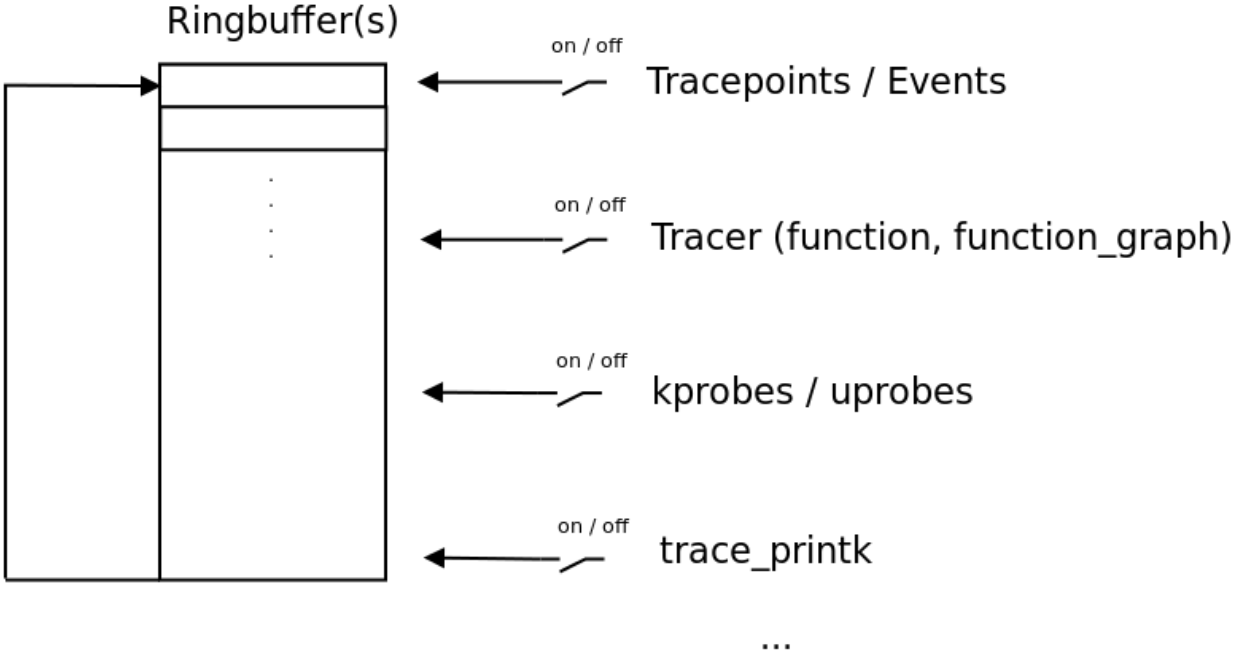
\includegraphics[width=0.7\linewidth]{figs/trace-overview.png}
%		\caption{trace-overview}
	\end{figure}


% 
\end{frame}
%------------------------------------------------
\begin{frame}[fragile]
    \frametitle{Event tracing}


    \begin{itemize}
        \item Pre-defined Events in the kernel
        \item Event groups
        \item Each event comes with several options
        \item Filtering based on event options
    \end{itemize}
% 
\end{frame}
%------------------------------------------------
\begin{frame}[fragile]
    \frametitle{Step by Step for Event tracing}


    \begin{itemize}
        \item Enable events
        \item Record a trace
        \item Analyze a trace
        \item Trace event format and filters
	    \begin{itemize}
	        \item Each trace event has a specific format and parameters.
          \item Put a filter on those parameters for recording a trace.
      \end{itemize}
    \end{itemize}
% 
\end{frame}
%------------------------------------------------
\begin{frame}[fragile]
    \frametitle{Tracing on multicore}


    \begin{itemize}
        \item One ringbuffer per cpu
        \item Trace contains ALL events
        \item The per\_cpu directory contains a trace for each cpu
        \item tracing\_cpumask can limit tracing to specific cores
    \end{itemize}
% 
\end{frame}
%------------------------------------------------
\begin{frame}
\frametitle{提纲} % Table of contents slide, comment this block out to remove it
\tableofcontents % Throughout your presentation, if you choose to use \section{} and \subsection{} commands, these will automatically be printed on this slide as an overview of your presentation
\end{frame}
%------------------------------------------------
\subsection{Tracers}

% 
%------------------------------------------------
\begin{frame}[fragile]
    \frametitle{Tracers}

% 
Available\_tracers contains the tracers which are enabled in the kernel configuration.

    \begin{itemize}
        \item function: Can turn all functions into trace events function\_graph: Similiar to function, but contains a call graph
        \item wakeup / wakeup\_rt: Measure the wakeup time for tasks / rt tasks
        \item irqsoff: useful for latency hunting. Identifies long sections with IRQs turned off
        \item  ...
    \end{itemize}
% 
\end{frame}
%------------------------------------------------
\begin{frame}[fragile]
    \frametitle{trace\_printk()}


    \begin{itemize}
        \item trace\_printk() can be used to write messages to the tracing ring buffer
        \item Usage is similar to printk()
    \end{itemize}
% 
\end{frame}
%------------------------------------------------
\begin{frame}[fragile]
    \frametitle{Tracing related kernel parameters}


    \begin{itemize}
        \item Set and start specified tracer as early as possible.
        \item Dump the tracing ring buffer if an Oops occurs. Using orig\_cpu it will only dump the buffer of the CPU which triggered the Oops.
        \item Only trace specific functions.
        \item Don't trace specific functions.
        \item Just enable trace events (comma separated list)
    \end{itemize}
% 
\end{frame}
%------------------------------------------------
\begin{frame}[fragile]
    \frametitle{Dynamic kernel tracepoints: KPROBES}


    \begin{itemize}
        \item Similar to Tracepoints
        \item Can be added / removed dynamically
        \item KPROBES for custom modules
	    \begin{itemize}
	        \item tracepoint for the function hello\_init
      \end{itemize}
    \end{itemize}
% 
\end{frame}
%------------------------------------------------
\begin{frame}[fragile]
    \frametitle{Dynamic Userspace Tracepoints: uprobes}


    \begin{itemize}
        \item Similar to kprobes
        \item For userspace applications
        \item A uprobe event is set on a specific offset in a userland process
        \item Powerful method to correlate your kernel and userland events!
    \end{itemize}
% 
\end{frame}
%------------------------------------------------
\begin{frame}
\frametitle{提纲} % Table of contents slide, comment this block out to remove it
\tableofcontents % Throughout your presentation, if you choose to use \section{} and \subsection{} commands, these will automatically be printed on this slide as an overview of your presentation
\end{frame}
%------------------------------------------------
\subsection{Graphical Front-end for Tracing Infrastructure}

% 
%------------------------------------------------
\begin{frame}[fragile]
    \frametitle{trace-cmd}


    \begin{itemize}
        \item trace-cmd is a commandline utility for controlling and analysing kernel traces.
        \item trace-cmd record generates a file called trace.dat.
        \item trace-cmd report uses the -i option for specifying an input file
        \item Recording traces via network
    \end{itemize}
% 
\end{frame}
%------------------------------------------------
\begin{frame}[fragile]
    \frametitle{Kernelshark: A graphical front-end}

% 
  \begin{figure}
    \centering
    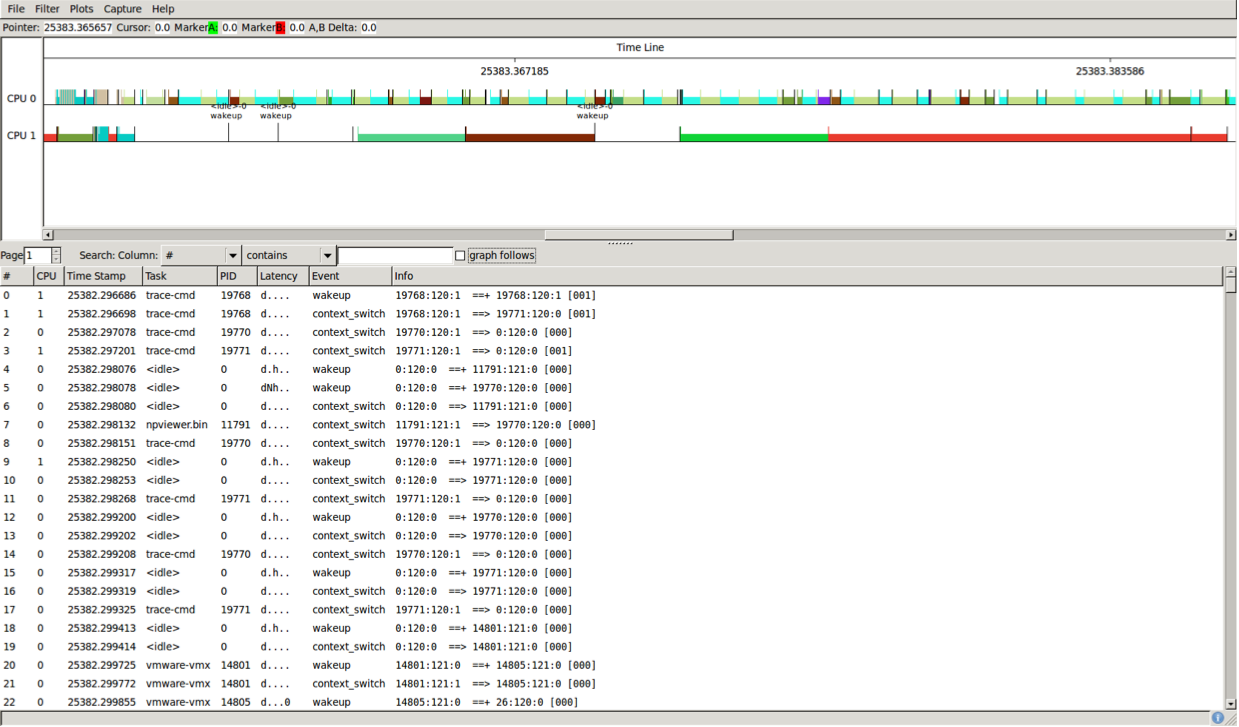
\includegraphics[width=0.75\linewidth]{figs/trace-kernelshark.png}
%		\caption{trace-kernelshark}
	\end{figure}


% 
\end{frame}
%------------------------------------------------
\begin{frame}[fragile]
    \frametitle{Tracecompass}


    \begin{itemize}
        \item Uses the Common Trace Format (CTF)
        \item perf can convert traces to CTF
        \item perf uses libbabeltrace for the convertion
        \item A recent version of libbabeltrace is needed
    \end{itemize}
% 
\end{frame}
%------------------------------------------------
\begin{frame}[fragile]
    \frametitle{Tracecompass}

% 
  \begin{figure}
    \centering
    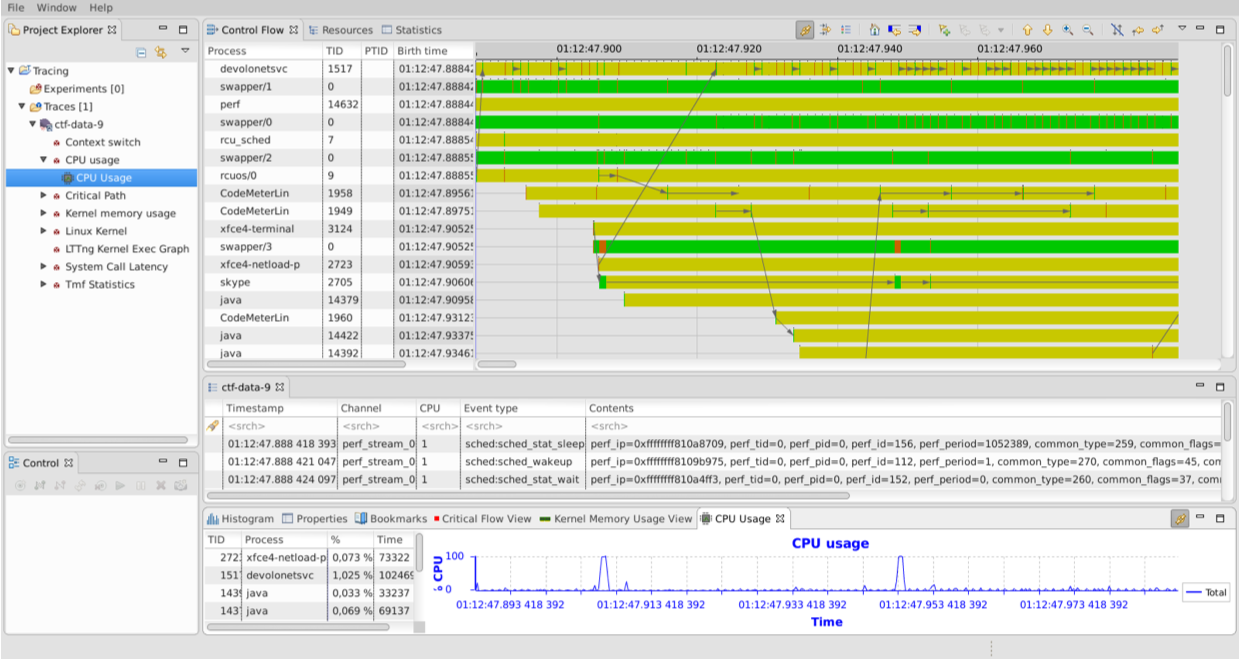
\includegraphics[width=0.8\linewidth]{figs/trace-tracecompass.png}
%		\caption{trace-tracecompass}
	\end{figure}

\end{frame}
%----------------------------------------------
%----------------------------------------------
\end{document}
